\section{Evaluation}
\label{sec:eval}
\subsection{Experimental Settings}
\textbf{Datasets.}
We validate \sysname on a dataset of $112$ participants ($35$ non-diabetes, $38$ type I diabetic patients, $39$ type II diabetic patients) collected during July 2016 to January 2017.
Each participant is equipped with a \TODO{concrete brand, type} CGM device to record blood glucose concentration every $3$ minutes and a smartphone with \sysname installed to collect external factor information either automatically (activities and sleep quality) or manually (food, drug, and insulin intake).
All participants agree to take measurements (\ie wear the CGM device and use \sysname to record external factors) for at least $5$ days.
In total we obtain \TODO{XXX} samples of blood glucose concentration and the corresponding external factors covering \TODO{XXX} hours.
In brief, we collect the following categories of data:
\begin{itemize}
  \item
  \textbf{Personal information.}
  We record basic personal data including gender, age, weight and health status as reference for user grouping.
  \tabref{tab:parcitipant} summarizes the basic information of the participants.
  \item
  \textbf{Blood glucose measurements.}
  Since we mainly aim to detect abnormal blood glucose events, we divide the blood glucose concentration into 4 levels: \TODO{the concrete range of each level}.
  The duration of blood glucose measurements varies from 5 to 30 days.
  \tabref{tab:bgdata} summarizes amount of blood glucose measurements.
  \item
  \textbf{External factor measurements.}
  During measurements of blood glucose concentration, each participant manually inputs the times of their daily meal, drug and insulin intake.
  \sysname automatically records activity levels and sleep quality as in \secref{subsec:external}.
  \TODO{show user interface?}
\end{itemize}

\begin{table}
  \centering
  \caption{Summary of participant information.}
  \label{tab:parcitipant}
  \subfloat[]{%
  \begin{tabular}{cc}
  \toprule
  \textbf{Age (year)} & \textbf{\# User} \\
  \midrule
  15-24 & 8 \\
  25-34 & 17 \\
  35-44 & 24 \\
  45-54 & 29 \\
  55-70 & 34 \\
  \bottomrule
  \end{tabular}}%
  \quad% --- set horizontal distance between tables here
  \subfloat[]{%
  \begin{tabular}{cc}
  \toprule
  \textbf{Weight (kg)} & \textbf{\# User} \\
  \midrule
  30-44 & 18 \\
  45-54 & 21 \\
  55-64 & 32 \\
  65-74 & 22 \\
  75-90 & 19 \\
  \bottomrule
  \end{tabular}}%
  \quad%
  \subfloat[]{%
  \begin{tabular}{cc}
  \toprule
  \textbf{Status} & \textbf{\# User} \\
  \midrule
  Non-diabetes & 35 \\
  Type I & 38 \\
  Type II & 39 \\
  \bottomrule
  \end{tabular}}
  \quad%
  \subfloat[]{%
  \begin{tabular}{cc}
  \toprule
  \textbf{Gender} & \textbf{\# User} \\
  \midrule
  Male & 57 \\
  Female & 55\\
  \bottomrule
  \end{tabular}}
\end{table}

\begin{table}
  \centering
  \caption{Summary of blood glucose measurements.}
  \label{tab:bgdata}
  \subfloat[]{%
  \begin{tabular}{cc}
  \toprule
  \textbf{Duration (days)} & \textbf{\# User} \\
  \midrule
  6-10 & 48 \\
  11-15 & 24 \\
  16-20 & 20 \\
  21-25 & 13 \\
  26-30 & 7 \\
  \bottomrule
  \end{tabular}}%
  \qquad% --- set horizontal distance between tables here
  \subfloat[]{%
  \begin{tabular}{cc}
  \toprule
  \textbf{Blood Glucose} & \textbf{\# Sample} \\
  \midrule
  Level 1 & 75369 \\
  Level 2 & 293530 \\
  Level 3 & 235686 \\
  Level 4 & 158054 \\
  Total & 762639 \\
  \bottomrule
  \end{tabular}}%
\end{table}

%\begin{table}[]
%  \centering
%  \caption{Summary of experimental settings.}
%  \label{tab:dataset}
%  \begin{tabular}{clccclcccccl}
%  \hline\hline
%  \multicolumn{12}{c}{\textbf{Blood Glucose}}                                                                                                                                                                                               \\ \hline
%  \multicolumn{2}{l}{\textbf{\cellcolor[gray]{0.8}Blood Level}} & \multicolumn{2}{r}{\textbf{\cellcolor[gray]{0.8}Level 1}} & \multicolumn{2}{c}{\textbf{\cellcolor[gray]{0.8}Level 2}} & \multicolumn{2}{c}{\textbf{\cellcolor[gray]{0.8}Level 3}} & \multicolumn{2}{c}{\textbf{\cellcolor[gray]{0.8}Level 4}} & \multicolumn{2}{c}{\textbf{\cellcolor[gray]{0.8}Total}} \\
%  \multicolumn{2}{l}{Number of Sample}     & \multicolumn{2}{c}{75369}            & \multicolumn{2}{c}{293530}           & \multicolumn{2}{c}{235686}           & \multicolumn{2}{c}{158054}           & \multicolumn{2}{c}{762639}         \\ \hline\hline
%  \multicolumn{12}{c}{\textbf{Experimental Duration}}                                                                                                                                                                                          \\ \hline
%  \multicolumn{2}{l}{\textbf{\cellcolor[gray]{0.8}Days}}        & \multicolumn{2}{c}{\textbf{\cellcolor[gray]{0.8}6-10}}    & \multicolumn{2}{c}{\textbf{\cellcolor[gray]{0.8}11-15}}   & \multicolumn{2}{c}{\textbf{\cellcolor[gray]{0.8}16-20}}   & \multicolumn{2}{c}{\textbf{\cellcolor[gray]{0.8}21-25}}   & \multicolumn{2}{c}{\textbf{\cellcolor[gray]{0.8}26-30}} \\
%  \multicolumn{2}{l}{Number of Users}      & \multicolumn{2}{c}{48}               & \multicolumn{2}{c}{24}               & \multicolumn{2}{c}{20}               & \multicolumn{2}{c}{13}               & \multicolumn{2}{c}{7}              \\
%  \hline\hline
%  \multicolumn{12}{c}{\textbf{Summary of participant data}}                                                                                                                                                                                      \\ \hline
%  \multicolumn{2}{l}{\textbf{\cellcolor[gray]{0.8}Age}}         & \multicolumn{2}{c}{\textbf{\cellcolor[gray]{0.8}15-24}}   & \multicolumn{2}{c}{\textbf{\cellcolor[gray]{0.8}25-34}}   & \multicolumn{2}{c}{\textbf{\cellcolor[gray]{0.8}35-44}}   & \multicolumn{2}{c}{\textbf{\cellcolor[gray]{0.8}45-54}}   & \multicolumn{2}{c}{\textbf{\cellcolor[gray]{0.8}55-70}} \\
%  \multicolumn{2}{l}{Number of Users}      & \multicolumn{2}{c}{8}                & \multicolumn{2}{c}{17}               & \multicolumn{2}{c}{24}               & \multicolumn{2}{c}{29}               & \multicolumn{2}{c}{34}             \\
%  \multicolumn{2}{l}{\textbf{\cellcolor[gray]{0.8}Weight}}      & \multicolumn{2}{c}{\textbf{\cellcolor[gray]{0.8}30-44}}   & \multicolumn{2}{c}{\textbf{\cellcolor[gray]{0.8}45-54}}   & \multicolumn{2}{c}{\textbf{\cellcolor[gray]{0.8}55-64}}   & \multicolumn{2}{c}{\textbf{\cellcolor[gray]{0.8}65-74}}   & \multicolumn{2}{c}{\textbf{\cellcolor[gray]{0.8}75-90}} \\
%  \multicolumn{2}{l}{Number of Users}      & \multicolumn{2}{c}{18}               & \multicolumn{2}{c}{21}               & \multicolumn{2}{c}{32}               & \multicolumn{2}{c}{22}               & \multicolumn{2}{c}{19}             \\
%  \multicolumn{4}{l}{\textbf{\cellcolor[gray]{0.8}Gender}}      & \multicolumn{3}{c}{\textbf{\cellcolor[gray]{0.8}Male}}                                                               & \multicolumn{5}{c}{\textbf{\cellcolor[gray]{0.8}Female}}                                                          \\
%  \multicolumn{4}{l}{Number of Users}      & \multicolumn{3}{c}{57}                                                                          & \multicolumn{5}{c}{55}                                                                       \\ \hline\hline
%  \multicolumn{12}{c}{\textbf{User Health Status}}                                                                                                                                                                                          \\ \hline
%  \multicolumn{3}{l}{\textbf{\cellcolor[gray]{0.8}Health Status}}                   & \multicolumn{3}{c}{\textbf{\cellcolor[gray]{0.8}Health}}                     & \multicolumn{3}{c}{\textbf{\cellcolor[gray]{0.8}Type I}}                      & \multicolumn{3}{c}{\textbf{\cellcolor[gray]{0.8}Type II}}                  \\
%  \multicolumn{3}{l}{Number of Users}                          & \multicolumn{3}{c}{35}                                  & \multicolumn{3}{c}{38}                                   & \multicolumn{3}{c}{39}                                \\ \hline
%  \end{tabular}
%\end{table}

\textbf{Ground Truth.}
We use the blood glucose concentrations collected by the CGM device as ground truth.

\textbf{Metrics.}
We mainly adopt three metrics to evaluate the performance of \sysname, including precision~\cite{}, recall~\cite{} and accuracy~\cite{}.

%
%
%\begin{table}[]
%\centering
%\caption{The details of dataset}
%\label{The details of dataset}
%\begin{tabular}{|l|c|c|c|c|l|}
%\hline
%\textbf{Blood Level}                  & \textbf{Level 1} & \textbf{Level 2} & \textbf{level 3} & \textbf{Level 4} & \textbf{Total}         \\ \hline
%\multicolumn{1}{|c|}{\textbf{Number}} & 75369            & 293530           & 235686           & 158054           & \multicolumn{1}{c|}{762639} \\ \hline
%\end{tabular}
%\end{table}

\subsection{Overall Accuracy}
Since all participants collected both measurements of CGM and external factors for at least 5 days, we use measurements during the former 4 days for training and the rest for testing.
\tabref{tab:confusion_matrix} shows the overall performance of \sysname.
All results are averaged over the testing data.
As shown, the recalls and the precisions for all the 4 blood glucose levels are above 79\% and 73\%, respectively.
In particular, the recalls for Level 1 (\TODO{low/high blood glucose?}) and Level 4 \TODO{low/high blood glucose?} are 83.13\% and 85.23\%, even though the training data for Level 1 and Level 4 only account for \TODO{XXX\%} and \TODO{XXX\%} of the entire training set.
Overall, \sysname yields an accuracy of 82.14\%.

\begin{table}[ht]
  \centering
  \caption{Confusion matrix of \sysname.}
  \label{tab:confusion_matrix}
  \begin{tabular}{|c|c|c|c|c|l|l|}
  \hline
  \multirow{2}{*}{\textbf{\begin{tabular}[c]{@{}c@{}}Ground\\ Truth\end{tabular}}} & \multicolumn{4}{c|}{\textbf{Predictions}}                                                                                 & \multicolumn{2}{l|}{\multirow{2}{*}{}}                                                            \\ \cline{2-5}
                                                                                 & Level 1                      & Level 2                      & Level 3                      & Level 4                      & \multicolumn{2}{l|}{}                                                                             \\ \hline
Level 1                                                                          & \cellcolor[gray]{0.8}62657                        & 5521                         & 3672                         & 3519                         & 83.13\%                             & \multirow{4}{*}{\rotatebox{90}{\textbf{Recall}} }                           \\ \cline{1-6}
Level 2                                                                          & 16346                        &  \cellcolor[gray]{0.8}240584                       & 27563                        & 9037                         & 81.96\%                             &                                                             \\ \cline{1-6}
Level 3                                                                          & 2660                         & 30905                        & \cellcolor[gray]{0.8}188472                       & 13649                        & 79.97\%                             &                                                             \\ \cline{1-6}
Level 4                                                                          & 3443                         & 5620                         & 14278                        & \cellcolor[gray]{0.8}134713                       & 85.23\%                             &                                                             \\ \hline
\multicolumn{1}{|l|}{\multirow{2}{*}{}}                                          & \multicolumn{1}{l|}{73.62\%} & \multicolumn{1}{l|}{85.12\%} & \multicolumn{1}{l|}{80.55\%} & \multicolumn{1}{l|}{83.72\%} & \multicolumn{2}{l|}{\multirow{2}{*}{\begin{tabular}[c]{@{}l@{}}Accuracy:\\ 82.14\%\end{tabular}}} \\ \cline{2-5}
\multicolumn{1}{|l|}{}                                                           & \multicolumn{4}{c|}{\textbf{Precision}}                                                                                 & \multicolumn{2}{l|}{}                                                                             \\ \hline
\end{tabular}
\end{table}

\subsubsection{Effectiveness of Features}
\tabref{tab:features} shows the average precisions and recalls for all the 4 blood glucose levels with different combinations of features.
By combining physiological features ($F_{p}$) with temporal features ($F_{t}$), the overall precisions and recalls improve by \TODO{XXX\% to XXX\%}.
\TODO{XXX feature brings in the most notable improvement in detecting abnormal blood glucose events (Level XXX and Level XXX).
This is because XXX.}

\begin{table}[h]
  \small
  \centering
  \caption{Effectiveness of features.}
  \label{tab:features}
  \begin{tabular}{|c|c|c|c|c|c|c|c|c|}
  \hline
                                   & \multicolumn{2}{c|}{\textbf{Level 1}}                     & \multicolumn{2}{c|}{\textbf{Level 2}} & \multicolumn{2}{c|}{\textbf{Level 3}}                     & \multicolumn{2}{c|}{\textbf{Level 4}}                     \\ \hline
  \textbf{Features}                  & \textbf{Precision} & \multicolumn{1}{l|}{\textbf{Recall}} & \textbf{Precision}  & \textbf{Recall} & \textbf{Precision} & \multicolumn{1}{l|}{\textbf{Recall}} & \textbf{Precision} & \multicolumn{1}{l|}{\textbf{Recall}} \\ \hline
  $F_{p}$                            & 43.37$\%$               & 32.82$\%$                                 & 46.03$\%$                & 39.10$\%$            & 51.79$\%$               & 48.95$\%$                                 & 56.30$\%$               & 43.49$\%$                                 \\ \hline
  $F_{p}$+$F_{t1}$                   & 51.97$\%$               & 58.11$\%$                                 & 60.42$\%$                & 58.90$\%$            & 63.35$\%$               & 53.59$\%$                                 & 69.82$\%$               & 55.16$\%$                                 \\ \hline
  $F_{p}$+$F_{t1}$+$F_{t2}$          & 64.60$\%$               & 73.08$\%$                                 & 69.87$\%$                & 61.23$\%$            & 74.33$\%$               & 67.81$\%$                                 & 76.64$\%$               & 72.32$\%$                                 \\ \hline
  $F_{p}$+$F_{t1}$+$F_{t2}$+$F_{t3}$ & 73.62$\%$   & 83.13$\%$                                 & 83.13$\%$               & 83.13$\%$            & 80.55$\%$   & 79.97$\%$
  & 83.72$\%$               & 85.23$\%$                                  \\ \hline
  \end{tabular}
\end{table}


\subsubsection{Effectiveness of Multi-task Framework}
To demonstrate the effectiveness of the multi-task framework in making full use of the training dataset, we compare \modelname with two other frameworks.
\begin{itemize}
  \item \emph{General Learning.}
  All the training data are directly fed into the model for training indifferently.
  General learning results in a \emph{generic} model that assumes universal correlations between all inputs and the blood glucose levels.
  \item \emph{Single Learning.}
  We train a different model for each individual participant by feeding his/her own measurements into the model.
  Single learning results in a \emph{personalized} model without sharing data and learning knowledge from measurements of other participants.
\end{itemize}
\figref{fig:cmp_model} shows the overall precisions and recalls of our multi-task learning framework as well as general learning and single learning.
As shown, our multi-task learning framework outperforms both general learning and single learning by \TODO{XXX\%} in precision and \TODO{XXX\%} in recall, respectively.
General learning performs slightly better than single learning for Level 2 and 3 (normal blood glucose levels), partly because the correlations between the inputs and normal blood glucose levels are relatively consistent for most people, while single learning suffers from lack of training data as it only uses user-specific data.
Conversely, single learning achieves higher precision and recall than general learning for Level 1 and 4 (abnormal blood glucose levels), partly because there are notable inter-person differences in the correlations between the inputs and abnormal blood glucose levels.
That is, the reasons for abnormal blood glucose levels can vary from person to person.
The multi-task framework combines the advantages of both general learning and single learning, which makes better use of the limited training data by sharing measurements among users, while preserving user-specific characteristics via the personal learning layer.
\begin{figure}[h]
  \centering
  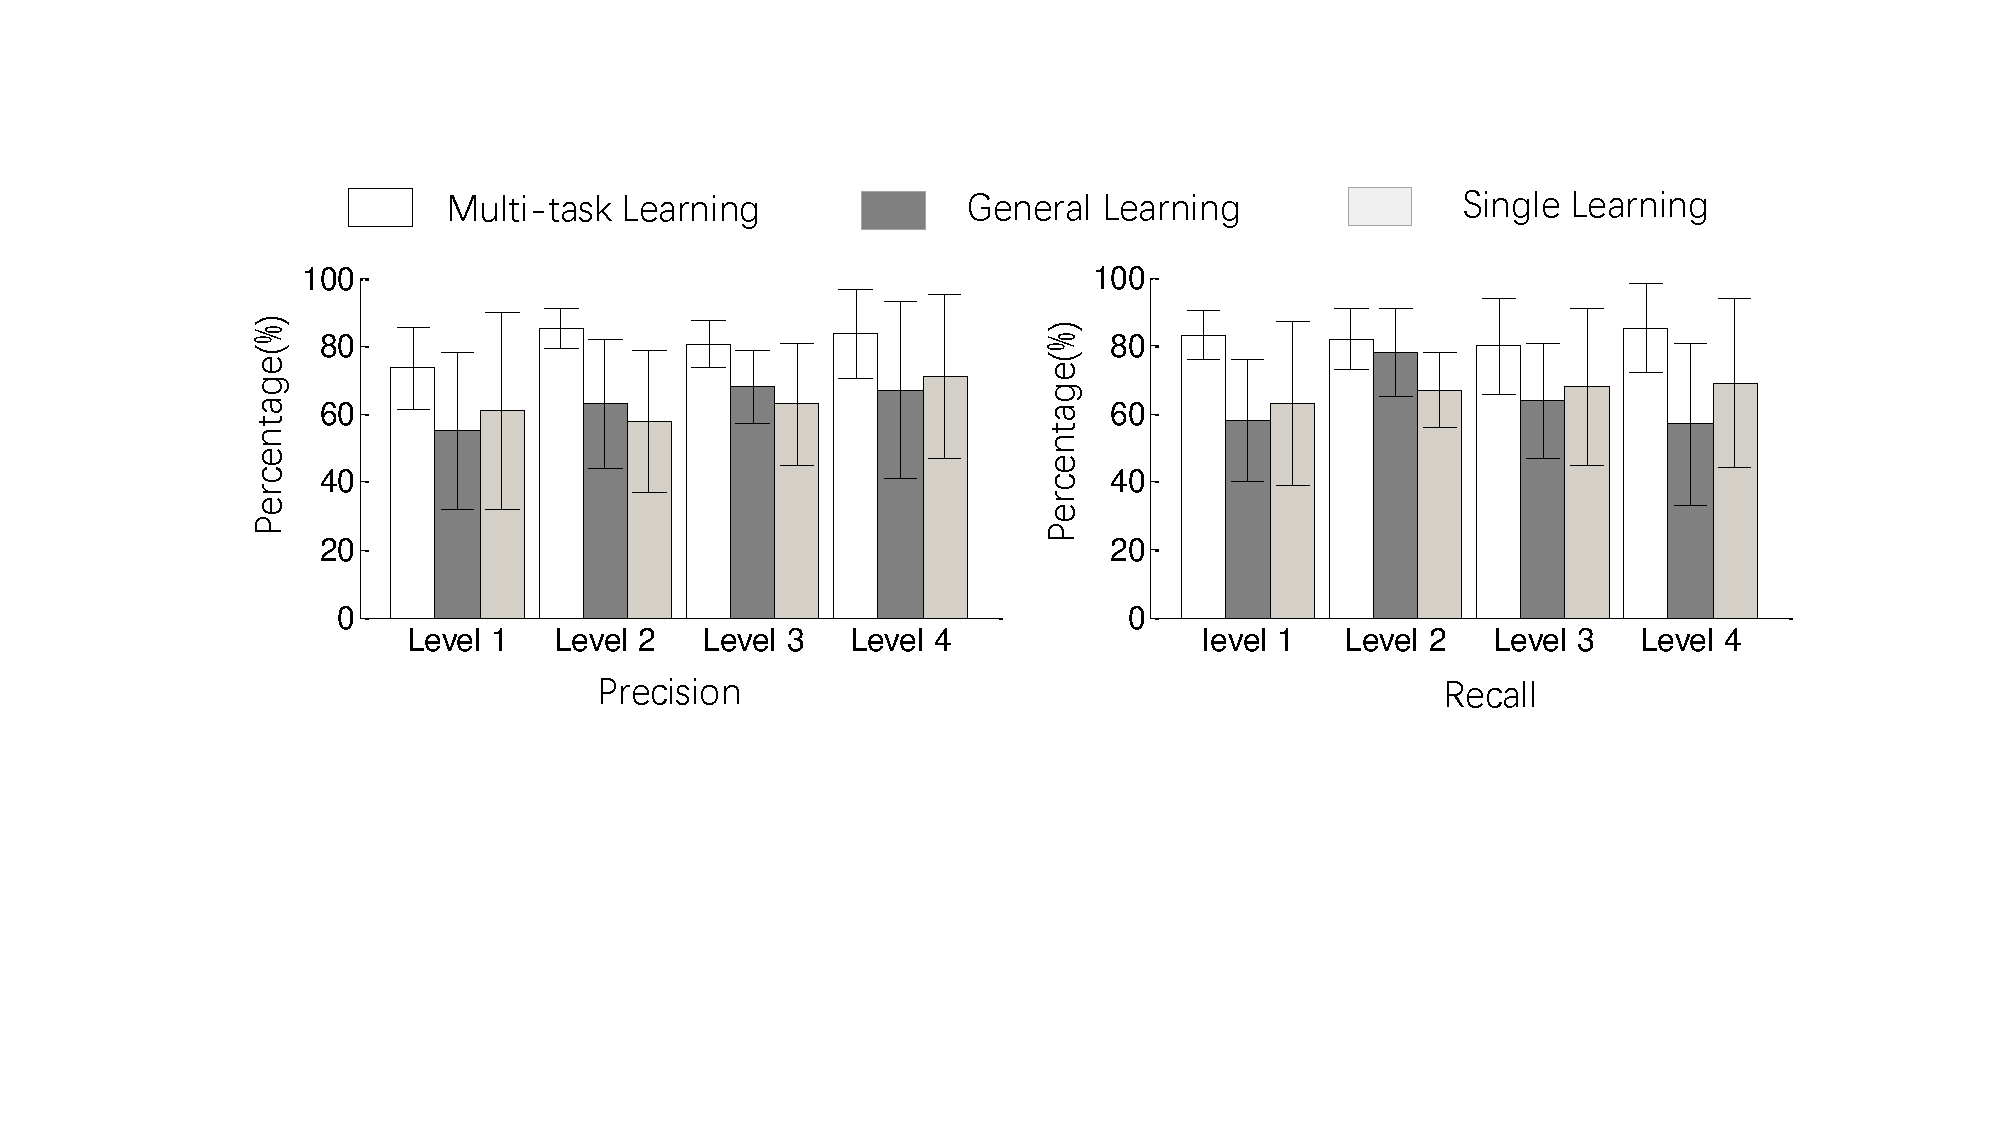
\includegraphics[width=0.9\columnwidth]{./img/CMP_Models.pdf}
  \caption{Effectiveness of our multi-task learning framework in making full use of the training dataset.}
  \label{fig:cmp_model}
\end{figure}



\subsubsection{Effectiveness of Deep Learning}
To demonstrate the effectiveness of adopting deep learning algorithms over conventional shallow learning algorithms, we compare our \modelname with the following mainstream learning algorithms.
\TODO{to complete and add the corresponding references}
\TODO{add a table summarizing the key parameters used for each model. Just mention the parameters for each model are optimized. No need to describe in such detail in the following.}
\begin{itemize}
  \item
  \textbf{Gradient Boosting (GB).}
  GB generates a prediction model by combining many weak classifiers into a stronger classification committee.
  We use AdaBoost procedure implemented in the fastAdaboost package to combine basic tree classifiers for ensemble learning.
  We vary the maximum tree depth from 10 to 50 by factors of ten.
  The number of boosting iterations is varied from 100 to 500 by a step size of 50.
  \item
  \textbf{Support Vehicle Machine (SVM).}
  SVM bases on the idea of ��optimal separating hyperplane�� that maximizes the separation margin of two data groups (classes).
  Due to this construction, it usually generalizes well, and its dual form is a quadratic programing that can be easily incorporated with kernels.
  We train the Gaussian kernel SVM classifier with the kernlab package, which implements the sequential minimal optimization algorithm.
  We vary the kernel width from $2^{-5}$ to $2^4$ with a factor of 2.
  We pick the penalty parameter from the set $\{10^i | i = -3, 0.5, 2\}$.
  To eliminate scale/location discrepancies among input variables, all features are normalized before being used in the training phase.
  \item
  \textbf{Hidden Markov model (HMM).}
  \item
  \textbf{Logistic Regression (LR).}
  LR models the posterior distribution of the class labels as a sigmoidal function of linear combinations of features.
  We use the glmnet package to train LR models with elastic net (combined L1 and L2) regularization.
  We vary the penalty parameter from 10$^{-3}$ to 10$^2$ with a factor 5.
  The mixing parameter is varied from 0 (Ridge) to 1 (Lasso) by a step size of 0.1.
  \item
  \textbf{Random Forest (RF).}
  As another ensemble method, RF combines many simple decision trees together and output the mode of classes for prediction.
  To avoid correlation among base trees, random set of features are selected in the splitting process when constructing each decision tree.
  For implementation, we adopt the conditional inference tree algorithm in the Party package.
  The total number of trees is tuned from 100 to 1000, and the maximum tree depth from 10 to 50.
  The splitting threshold is also varied from 0.1 to 0.9 with 0.1 intervals for cross validation.
  \item
  \textbf{Gaussian Processes (GP).}
  Instead of directly parameterizing a latent function for classification, GP models it with a generic Gaussian process.
  The posterior of the process is updated with training data set, and is ��squashed�� through a logistic function for classification.
  We implement GP with the kernlab package, which includes several approximation algorithms for acceleration.
  We use the radial basis kernel and vary the kernel width from 2$^{-5}$ to 2$^4$ with an incremental factor of 2$^{0.5}$.
\end{itemize}
\TODO{results}

\subsection{Micro-benchmarks}
In this section we evaluate the performance of \sysname for different participant groups as well as its temporal performance.

\subsubsection{Impact of amount of training samples}
In this experiment, we evaluate the performance of \sysname with increasing numbers of training samples.
Since our dataset consists of measurements of durations from 5 to 30 days (see \tabref{tab:bgdata}), we use measurements of 5 to 25 days for training and the remaining 5 days for testing.
The results are averaged over all testing samples as in previous evaluations.
\figref{fig:per_under_train_days} illustrates the results for all the 4 blood glucose levels.
As expected, the precisions and recalls for all the 4 blood glucose levels improve smoothly with the increase of training samples.
The results verify that the challenge (and our motivation to adopt a multi-task learning framework) is the lack of training data.
Note that \sysname is not a replacement of the current CGM devices, but rather, a complement when CGM devices are uncomfortable or inconvenient to wear.
Therefore we envision the training dataset will grow gradually after multiple times of CGM device wearing, at least for diabetes patients, and the overall accuracy will also improve over time as a result.

\begin{figure}[h]
  \centering
  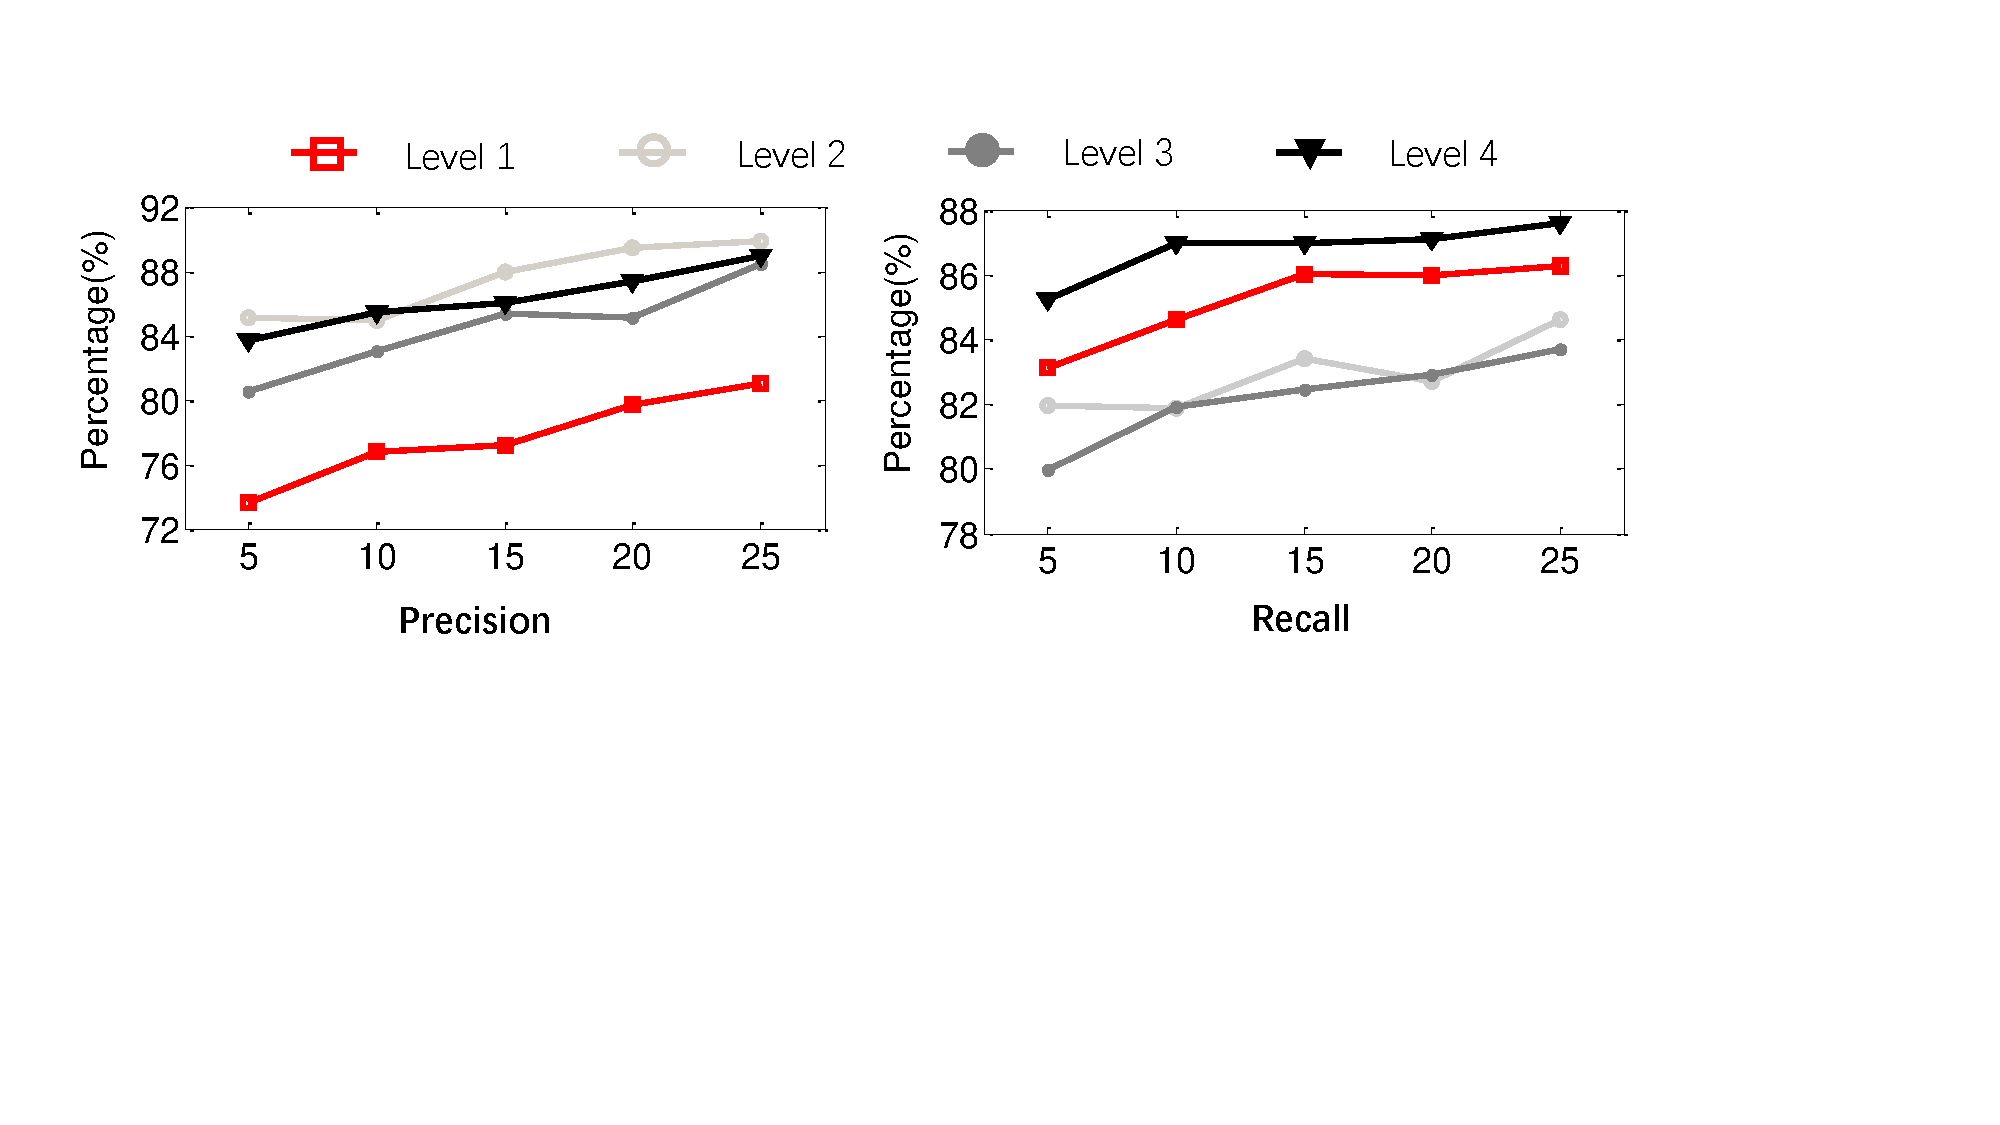
\includegraphics[width=0.9\columnwidth]{./img/performance_under_days.pdf}
  \caption{Impact of increasing amount of training samples.}
  \label{fig:per_under_train_days}
\end{figure}

\subsubsection{Impact of Temporal Gaps}
The blood glucose concentration is correlated with the previous blood glucose concentration because of the control loop of the glucose metabolism~\cite{bib:TBE07:Dalla, bib:PE04:Hovorka, bib:IJNMBE16:Oviedo}.
Since \sysname does not rely on the previous blood glucose level as an input, it is natural that the accuracy of \sysname will degrade if there is a long gap between the training and the testing datasets (\ie the training dataset can be outdated).
\figref{fig:per_under_various_pred_days} plots the overall performance by training using the same 4 days of measurements, and testing on measurements collected on the 5-9th, 10-14th, 15-19th, 20-24th, and 25-29th days, respectively.
As expected, both the precisions and recalls drop moderately with the increase of temporal gaps between the training and the testing datasets, with a maximum decrease of \TODO{XXX\%} and \TODO{XXX\%} in precision and recall after XXX days.
From the results, we recommend \sysname users to put on the CGM device to \TODO{retrain the model?} at least every three weeks (?).

\begin{figure}[h]
  \centering
  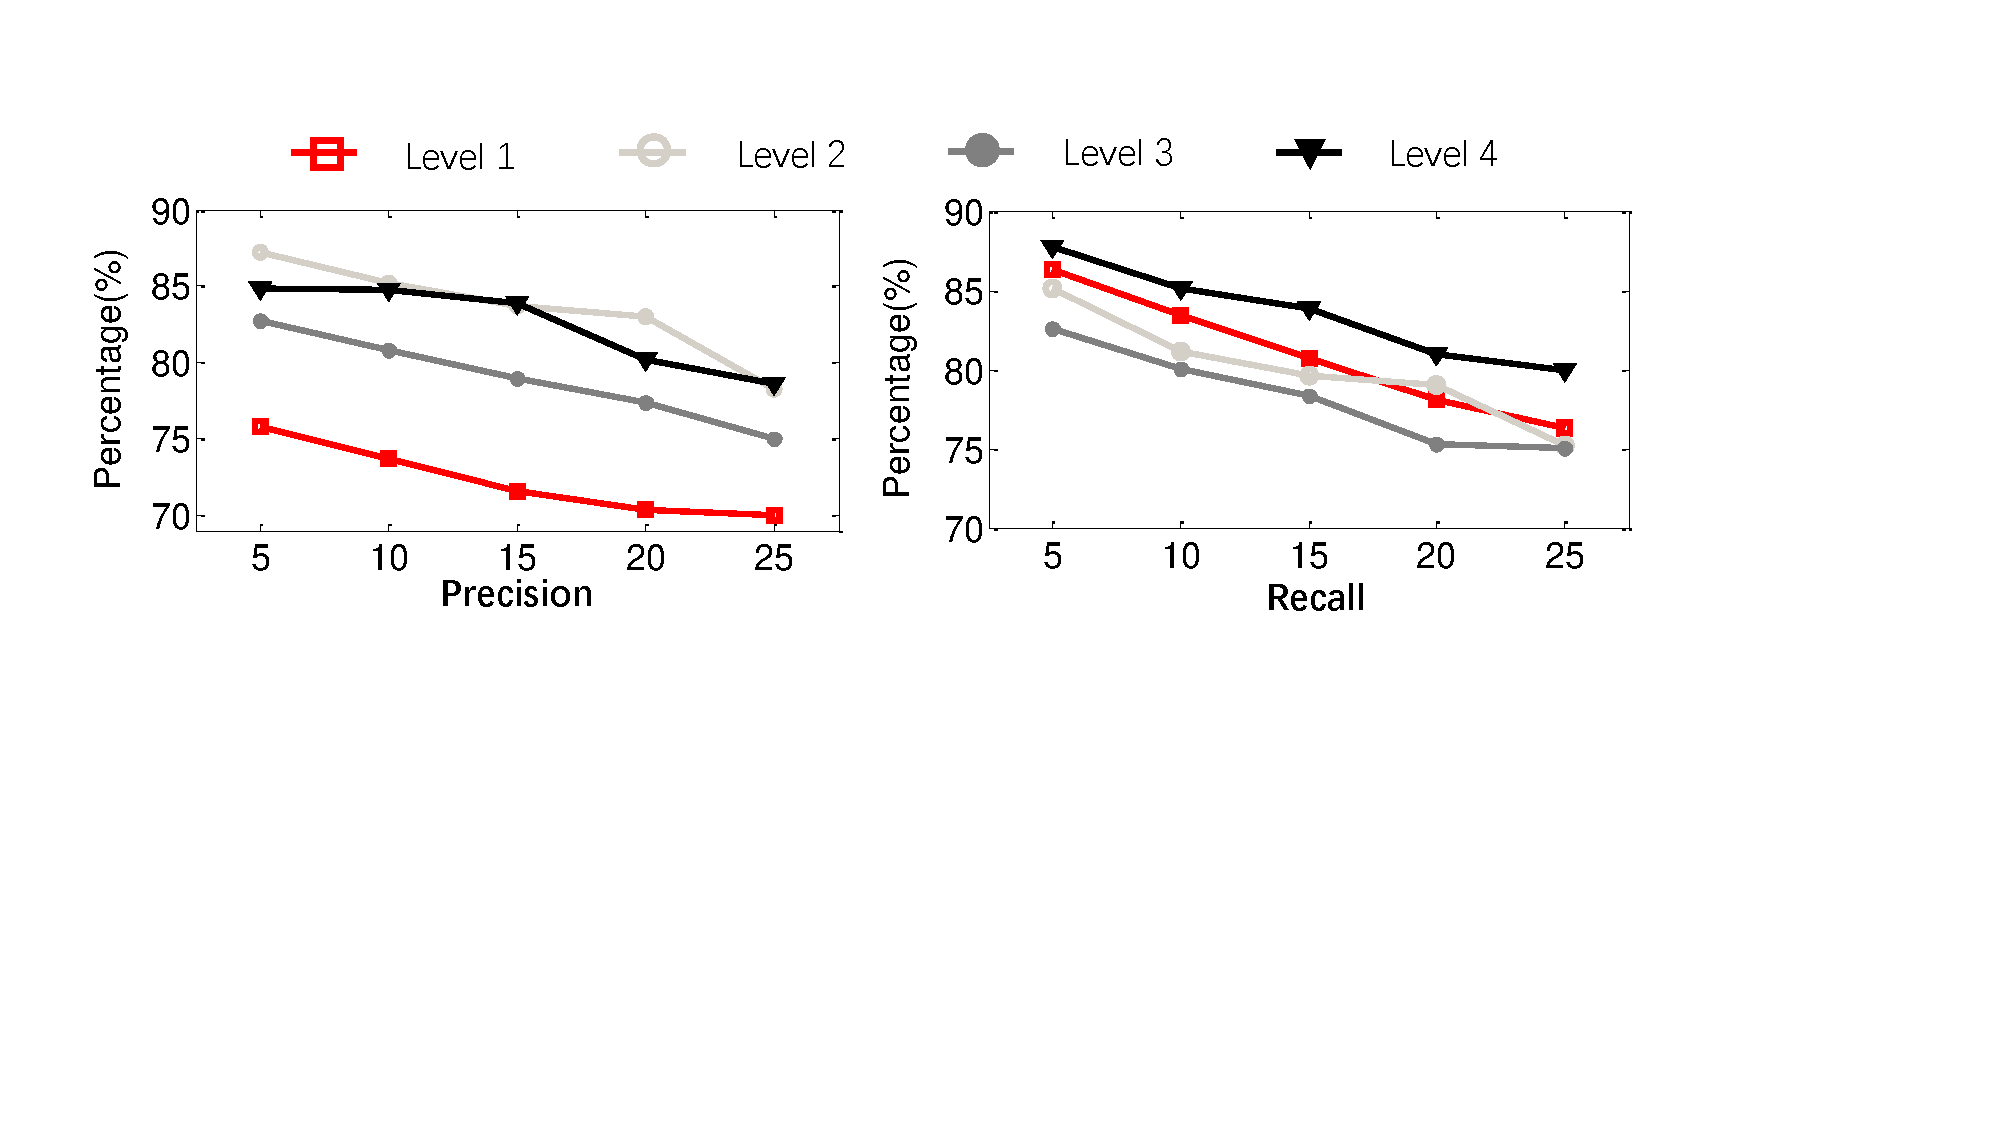
\includegraphics[width=0.9\columnwidth]{./img/Performance_gap.pdf}
  \caption{Impact of temporal gaps between the training and testing datasets.}
  \label{fig:per_under_various_pred_days}
\end{figure}


\subsubsection{Detection Accuracy throughout a Day}

\figref{fig:pre_gt} compares the predictive results of \sysname and true blood glucose level of a user over one day.
\TODO{redraw similar figures for a non-diabetic user, a type I user and a type II user}.
\TODO{better to include a trace where the accuracy when taking exercises, taking drugs and foods, is high. Also need to explain what the user is doing when the prediction is wrong.}

\begin{figure}[h]
  \centering
  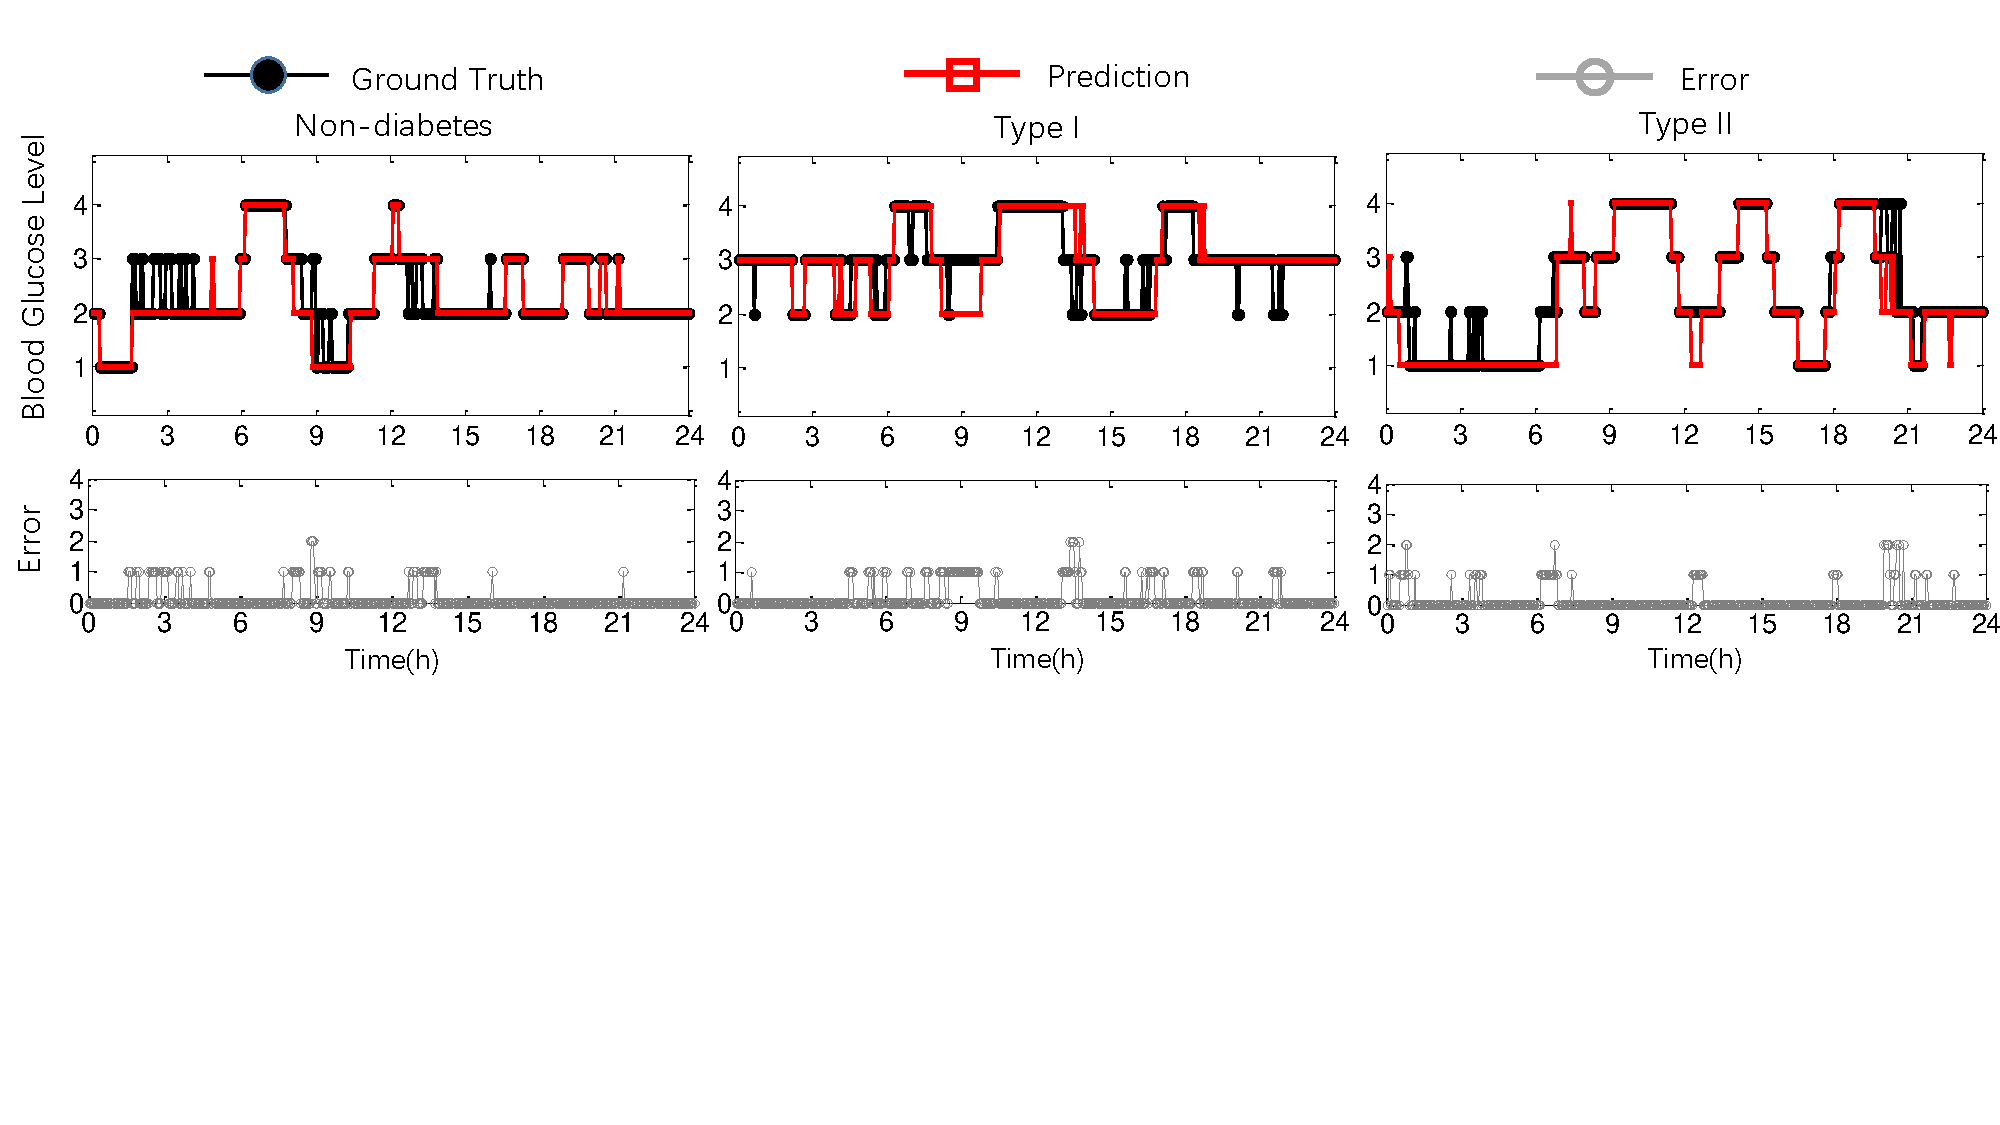
\includegraphics[width=0.5\columnwidth]{./img/pred_vs_gt.pdf}
  \caption{The comparison of prediction and the ground truths of one user.}
  \label{fig:pre_gt}
\end{figure}

\subsubsection{Detection Accuracy for Different Groups}

\TODO{redraw the figures, no need to include general and personal learning here. show the performance for different health status, gender, age groups, weight groups, \etc, explain why \sysname works better for certain groups, or works well for all groups}.

We also apply general learning approach on the users in same group, and compare the prediction performance of \modelname. Fig.~\ref{fig:cmp_groups}
shows the results. As is shown, \modelname outperforms the general learning methods in each group, especially the performance of level 1 and level 4. It mainly results by two reasons. On the one hand, the limitation of blood glucose data in each group weakens the capability of temporal dynamic characteristics. On the other hand, the imbalanced distribution of blood glucose data of one group also low the performance down. For example, much more data of level 4 and much less data of level 1 in group 3 (type II diabetes) low down the recall of level 1 and the precision of level 4. It is even hard to be solved by the cost sensitive approach.


\begin{figure}[!t]
\centering
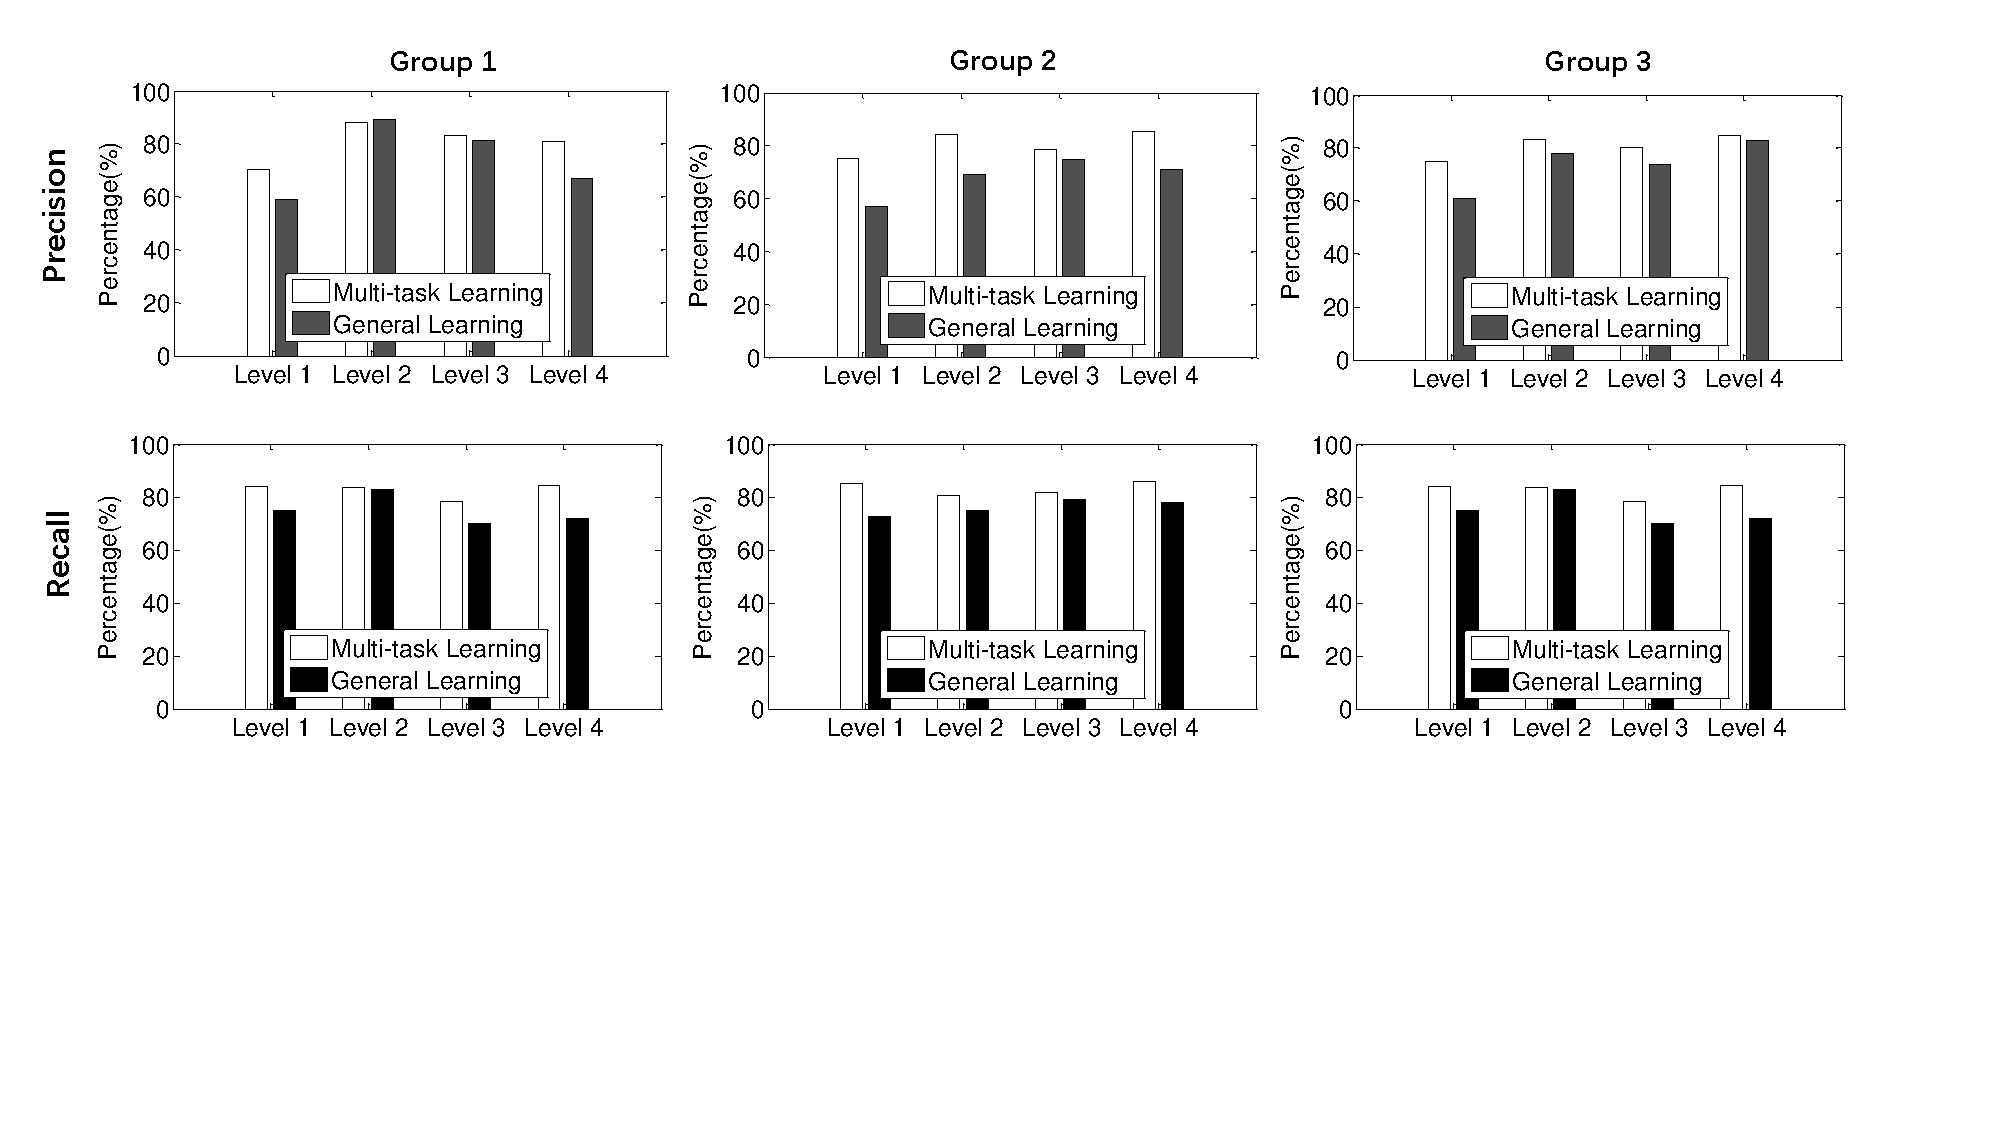
\includegraphics[width=0.9\columnwidth]{./img/group_multi_task.pdf}
\caption{The comparison of multi-task learning and group general learning.}
\label{fig:cmp_groups}
\end{figure}

